\chapter{Dataset Building}
\label{cha:4}

\section{BAT dataset}

\subsection{Characteristics} \label{bat-characteristics}

The BAT dataset \cite{spinde-2023-bat} is chosen instead of NLPCSS \cite{chen-etal-2020-nlpcss} for this project due to its article-level suitability and labels fluidity, as well additional metadata as it contains outlets information. It contains 6345 rows of manually labeled news articles from 255 English-speaking news outlets (US-based), originally scraped from Ad Fontes Media's website along with their respective \textbf{political bias} and \textbf{reliability scores}. Articles in the dataset encompassed a wide arrange of topics such as COVID-19, politics, and lifestyle. The political bias score measures the extent of political influence, ranging from -42 (most extreme left) to +42 (most extreme right). The reliability score reflects the article's truthfulness, with values ranging from 0 (least reliable, containing inaccurate or fabricated information) to 64 (most reliable, original fact reporting). However, since this dataset depends on manual labeling, the selection of articles by Ad Fontes Media likely introduces bias into the dataset \cite{spinde-2023-bat}.

Both political bias and reliability scores on each article were rated using defined metrics and multiple sub-factors, performed by three randomly selected analysts from Ad Fontes Media's team of over 60 experts. The corresponding three scores were then averaged, producing the final article scores. Moreover, each group consists analysts with different beliefs in the political spectrum i.e., left, center, and right.

The reliability score evaluates original fact reporting to analysis, opinion, propaganda, and inaccurate/fabricated information, with scores above 40 generally considered good and scores below 24 typically seen as problematic, scores between 24 and 40 suggest a variety of factors, including a strong presence of opinion and analysis or significant variability in reliability across different articles \cite{adfontes}. This metric is chosen as the main label in this project due to its correlation with textual-level bias: phrasing bias, spin bias, and statement bias described in \ref{media-bias-definition}


\subsection{Extension}

The original BAT dataset only contains news titles and links (along with other metadata) and is missing the body content of articles. To overcome this, a Python script is written and executed, iteratively visiting each of the URL from the dataset and scrape the news content. This was not an easy task as each website has its own unique structures and formats. Furthermore, the scraped text contains noises that are almost impossible to remove through the script. Some outlets such as The Nation, Chicago Tribune, and Truthout required manual intervention as the scraped text were duplicated over themselves. The current extended dataset contains 5270 rows of articles, mainly due to unavailable websites and missing articles.

To remove noises from article content, the text are then pre-processed extensively. All the content of every article in the dataset were joined into one single list, split into words, and then compared against an English word list (cite), resulting in a list of faulty words sorted by their occurences. Using this list, noisy patterns were analysed and handled through a combination of string and regex methods, conjoined words identified and fixed through a giant Python dictionary. This process is repeated more than several times until contents are valuable enough to work with. Note that at this point some noises still remain within the text as it will take an extensive amount of time and manual labour to completely clean the text.

\begin{comment}
Explain further on preprocessing scraped text. More details on the preprocessing scripts?
\end{comment}

\subsection{Analysis}

\begin{figure}[ht]
    \centering
    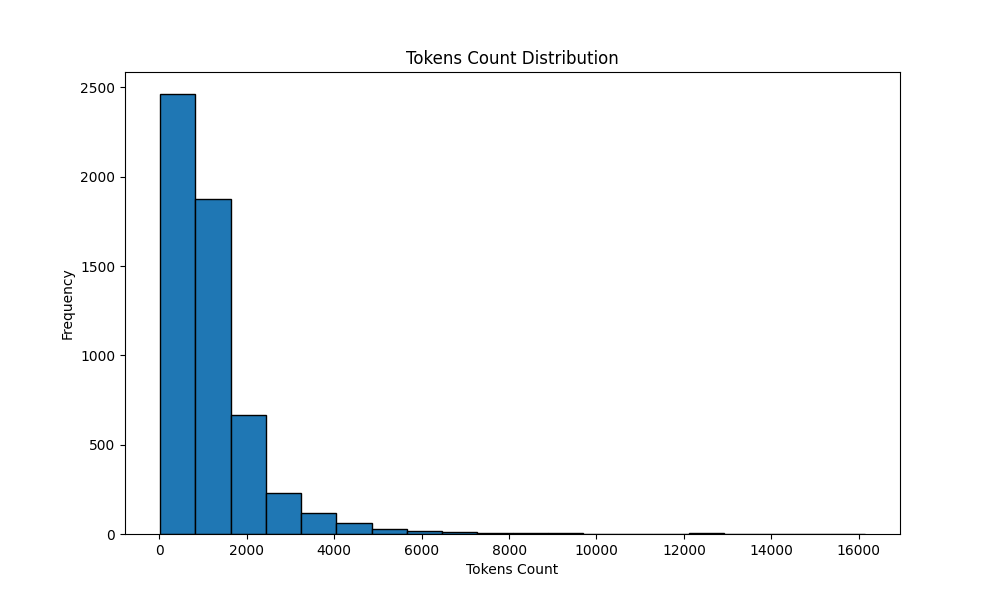
\includegraphics[width=0.9\linewidth]{figures/tokens_count_vx_hist.png}
    \caption{Articles tokens count distribution}
    \label{fig:tokens_hist}
\end{figure}

\begin{figure}[ht]
    \centering
    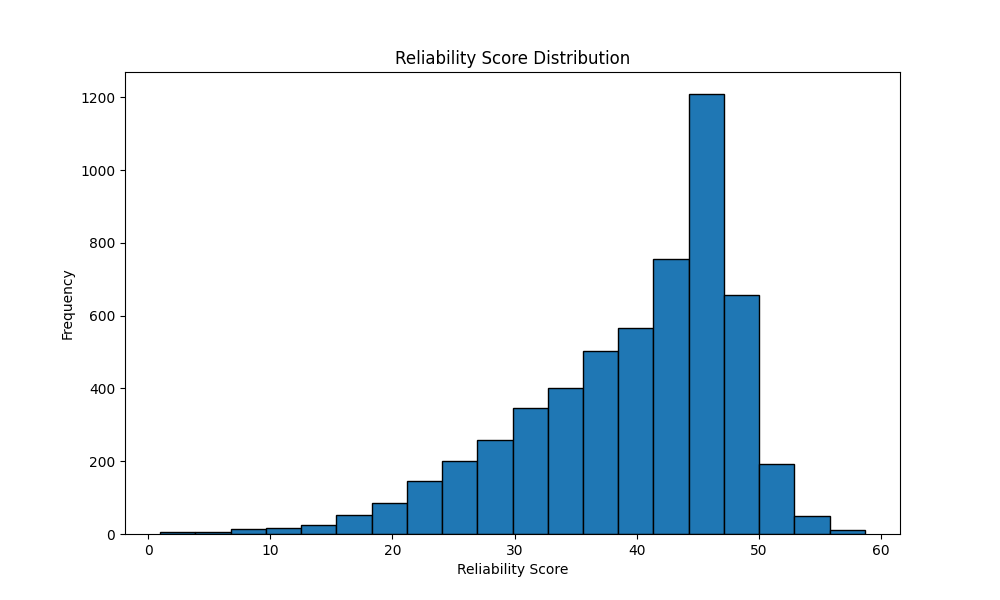
\includegraphics[width=0.9\linewidth]{figures/reliability_score_hist.png}
    \caption{Reliability score distribution}
    \label{fig:reliability_score_hist}
\end{figure}

The article contents tokens length ranges between 22 tokens up to 15530 tokens, with an average length of 1186.5 and a median value of 887 tokens. Only 9 articles have more than 10000 tokens, while there are 106 of articles with less than 100 tokens. Furthermore, only 1193 articles stay between 512 tokens, which is the limit for BERT input. Articles reliability score ranges from 1.0 to the 58.67, the majority have value between 20 - 50. Not a single articles were rated more than 60 despite the highest score being 64. Visualisations can be seen in both Figure \ref{fig:tokens_hist} and Figure \ref{fig:reliability_score_hist}, as well as Figure \ref{fig:tokens_hist_split}


\begin{figure}[ht]
    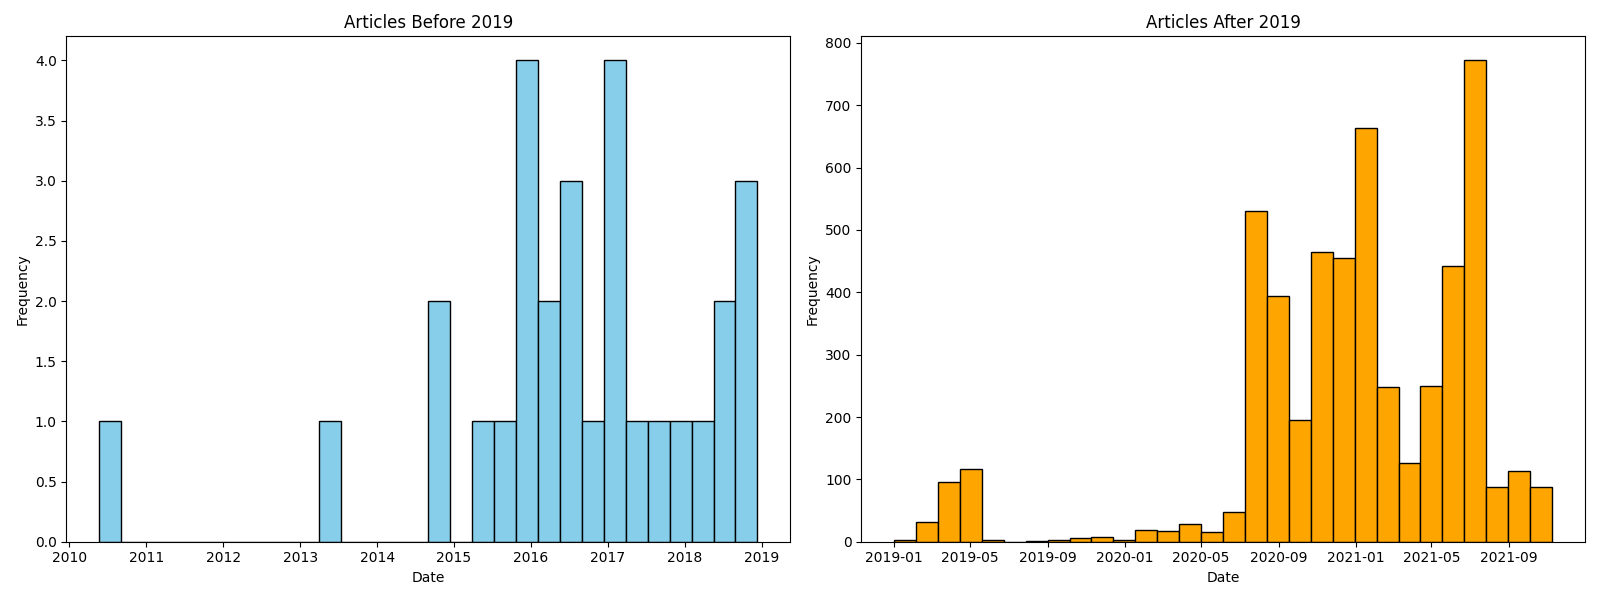
\includegraphics[width=0.9\linewidth]{figures/dates_hist.png}
    \caption{Article dates distribution}
    \label{fig:dates_hist}
\end{figure}

Most articles are written and published within the last 6 years, with only 29 articles, a minuscule percentage, published before 2019, shown in Figure \ref{fig:dates_hist}. From my personal analysis, these 29 articles generally contain similar topics to articles published after 2019 and therefore should not hold any difference in behaviour and characteristics.


\begin{figure}[ht]
    \centering
    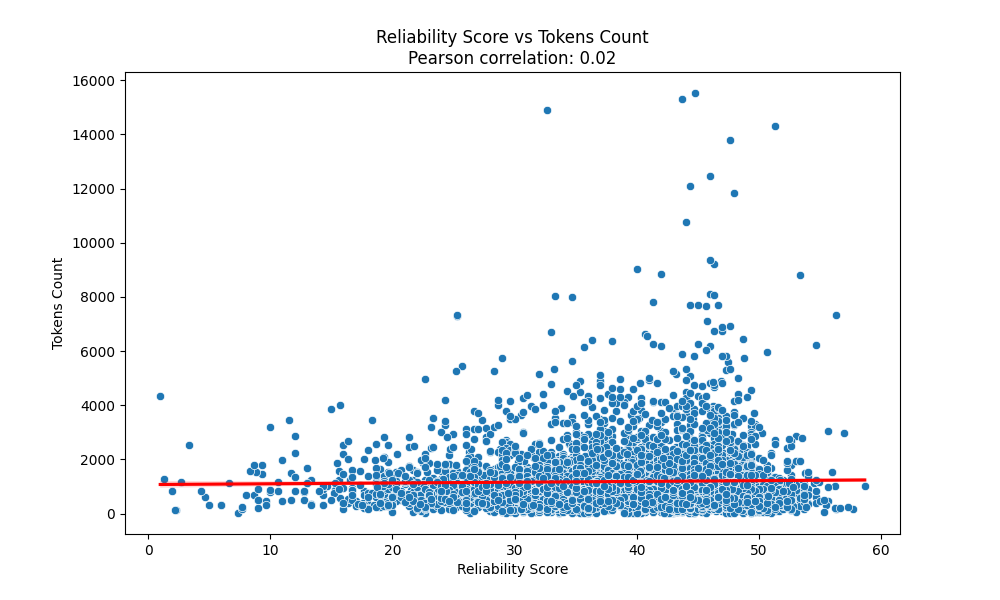
\includegraphics[width=0.9\linewidth]{figures/correlation_tokens_reliability_score.png}
    \caption{Pearson correlation between tokens count and reliability score}
    \label{fig:pearson_correlation}
\end{figure}


Figure \ref{fig:avg_tokens_count_per_class} shows that all classes seem to have similar tokens count, close to the overall average. Class 'Problematic' and 'Questionable', being the two most biased classes, seem to have lower average tokens count than the two other classes. However, further analysis (Figure \ref{fig:pearson_correlation}) shows that there is virtually no linear relationship between between tokens count and reliability score, with a Pearson correlation coefficient is 0.02. This proves that the length of an article has no significant impact with its reliability score. In other words, longer articles are not necessarily more or less reliable than shorter ones based on the provided data.

\begin{comment}
relationship between words and reliability score?
\end{comment}


% \section{Conclusion}
% The final section of the chapter gives an overview of the important results
% of this chapter. This implies that the introductory chapter and the
% concluding chapter don't need a conclusion.


%%% Local Variables: 
%%% mode: latex
%%% TeX-master: "thesis"
%%% End: 
